\documentclass[a4paper]{article}

%% Language and font encodings
\usepackage[english]{babel}
\usepackage[utf8x]{inputenc}
\usepackage[T1]{fontenc}

%% Sets page size and margins
\usepackage[a4paper,top=3cm,bottom=2cm,left=2cm,right=4cm,marginparwidth=3cm]{geometry}

%% Useful packages
\usepackage{amsmath}
\usepackage{bm}
\usepackage{amssymb}
\usepackage{float}
\usepackage{graphicx}
\usepackage{mathtools}
\usepackage[colorinlistoftodos]{todonotes}
\usepackage[colorlinks=true, allcolors=blue]{hyperref}
\renewcommand{\familydefault}{\sfdefault}
\usepackage{hyperref}

\newcommand{\introduce}[1]{%
  \leavevmode % if at the start of a paragraph 
  \marginpar{\small\emph{#1}}% the note
}

\newcommand{\ix}[1]{%
  \leavevmode % if at the start of a paragraph 
  \marginpar{\small\emph{#1}}% the note
}
\newcommand{\expt}[1]{%
  \mathbb{E}[#1]
}

\newcommand{\vect}[1]{\boldsymbol{\mathbf{#1}}}
\DeclarePairedDelimiter{\mybrace}{\lbrace}{\rbrace}
\DeclarePairedDelimiter{\magn}{|}{|}

\title{\textbf{3F3 Statistical Signal Processing: First Draft}\\
\textit{`Need to Know...'}
}
\author{Mrinank Sharma}

\begin{document}
\maketitle
% \tableofcontents

This is an attempt to condense everything which \textbf{must be memorised} for this course and hence does not include data-book content. However, more involved proofs are included here.
\begin{enumerate}
\item\introduce{Probability Space}We call $(\Omega, P)$ the \emph{probability space} where $\Omega$ is the sample space (the set of all possible outcomes) and $P$ is a mapping from events to a number in the interval $[0,1]$.

\item\introduce{Probability Axioms} A probability $P$ assigns each event $E, E\subset \Omega$, a number in $[0,1]$. $P$ must satisfy the following axioms.
\begin{itemize}
\item $P(\Omega)=1$.
\item For disjoint $A_1, A_2, ...$ we can state $P(\bigcup\limits_{i=1}^{\infty} A_i)=\sum_{i=1}^\infty P(A_i)$
\end{itemize}
All the rules of probability follow from the above axioms. It is often useful to draw Venn diagrams.

\item\introduce{Indicator Function}Define the indicator function for an event $E$.
\begin{align*}
\mathbb{I}_E(t) = \begin{cases}
1\ \ &t\in E\\
0 &t\notin E
\end{cases}
\end{align*}

\item\introduce{Conditional Probability}Conditional probabilities are themselves proper probability distributions and follow the axioms of probability (by considering $P(\Omega |G)$ and $P(A\cup B|G)$ for disjoint $A, B$). The above definition gives rise to the probability chain rule. 

\item\ix{Independent Events}For independent events, 
\begin{equation*}
P(A,B) = P(A \cap B) = P(A)P(B) \Leftrightarrow P(A|B)=P(A)
\end{equation*}

\item\ix{Random Variable Definition}Given a probability space, $(\Omega, P)$, a random variable is a function $X: \Omega\rightarrow\mathbb{R}$. There is a sample space behind every random variable and the probabilities depend both on the probability space and the mapping. 

\ix{Discrete RV}A random variable is discrete if its range is a finite or countable set. A set is countable if a one-to-one mapping from the set to the integers can be defined. For these variables a \textbf{probability mass function} is used.

\ix{Continuous RV}Continuous random variables have probability density functions, not mass functions. For these variables there must exist a non-negative function, $f_X(x)$ such that $\int_{-\infty}^{\infty}f_X(x)\ dx=1$ and for $a<b$, $Pr(a\leq X\leq b)=\int_a^bf_X(x)\ dx$. A continuous RV has no concentration of probability at particular points; the probability of a single value is meaningless. 

\item\ix{Cumulative Density Function}The CDF is defined as 
\begin{equation*}
F_X(x) = Pr(X\leq x)
\end{equation*}
From the axioms of probability, the following properties hold. 
\begin{itemize}
\item $0\leq F_X(x) \leq 1$.
\item $F_X(x)$ is non-decreasing as x increases.
\item $Pr(x_1 < X\leq x_2) = F_X(x_2) - F_X(x_1)$.
\item $\lim_{x\rightarrow -\infty}F_X(x)=0$ \& $\lim_{x\rightarrow \infty}F_X(x)=1$
\item $F_X(x)$ is right-continuous. 
\end{itemize}
For a continuous RV, 
\begin{align*}
F_x(x) = \int_{-\infty}^x f(t)\ dt\ \ \ f_X(x)=\frac{dF_X(x)}{dx}
\end{align*}

\ix{CDF Method for Transforming RV}The CDF can be used to transform random variables. Let $X$ be a random variable and let $Y=r(X)$. 
\begin{enumerate}
\item Find the set $A_y=\left\lbrace x: r(x)\leq y\right\rbrace$.
\item Find the CDF of Y.
\begin{align*}
F_Y(y) &= Pr(r(X)\leq y) = Pr(X\in A_y)\\
&= \int_{-\infty}^{\infty}\mathbb{I}_{A_y}f_X(x)\ dx
\end{align*}
\item Differentiate to form the probability density function.
\end{enumerate}

\item\ix{Sum of independent RV}The probability density function of the sum of two independent random variables is the convolution between their probability density functions.
$f_Y(y)=\int_{-\infty}^{\infty}f_1(x_1)f_2(y-x_1)\ dx_1$

\item\ix{Rule of Iterated Expectation}For random variables $X$ and $Y$,
\begin{align*}
\mathbb{E}_{X,Y}[r(X,Y)] = \mathbb{E}_{Y}[\mathbb{E}_{X}[r(X,Y)|Y]]
\end{align*}

\item\ix{Expection of the Product of Independent RVs}
For independent $X_1, X_2, ..., X_n$
\begin{align*}
\mathbb{E}[\Pi_{i=1}^{n}X_i] = \Pi_{i=1}^{n}\mathbb{E}[X_i]
\end{align*}
This result can be shown by expanding the expectation formula and factorising the joint pdf. 

\item\ix{Sum of RVs}For \textbf{any }$X_1, X_2, ..., X_n$
\begin{align*}
\mathbb{E}[\sum_{i=1}^{n}X_i] = \sum_{i=1}^{n}\mathbb{E}[X_i]
\end{align*}
To prove this, write the expectation as an integral. 

\item\ix{Jacobian}For one-to-one or many-to-one mappings, the \emph{Jacobian} can be used to calculate transformed probability densities. For a transformation with \textbf{random vectors} $\vect{x}, \vect{y}$ and $\vect{y}=G(\vect{x})$  The Jacobian can be expressed as follows:
\begin{align*}
f_Y(\vect{y})=\sum_{i}f_x(G^{-1}_i(\vect{y}))||\vect{J}|| \ \ \ |\vect{J}|=\frac{\partial(x_1, ..., x_n)}{\partial(y_1, ..., y_n)}
\end{align*}
where $||\vect{J}||$ is the modulus of the Jacobian matrix and serves to normalise the density. The form of the Jacobian can be recalled (in a hand-wavey manner) by noting that $f_y dy = f_x dx$ and extending this to vectors.

\item\ix{Characteristic Function}Define the characteristic function of a random vector, $\vect{x}$ as follows
\begin{align*}
\varphi(\vect{t}) = \mathbb{E}[exp(j\vect{t}^T\vect{x})],\ \ \vect{t}\in\mathbb{R}^n
\end{align*}
The characteristic function fully defined the probability distribution (there is a one-to-one mapping, e.g. Fourier transforms). The characteristic function is useful for calculating $\mathbb{E}[X^N]$ (for a random variable, consider differentiating the characteristic function and substituting $t=0$).

For the sum of independent random variables, the overall characteristic function is the product of each characteristic function (by expectation of the product of independent random variables).

\item\ix{Markov Chains}Let the process $\left\lbrace X_n \right\rbrace_{n\geq 0}$ be a collection of discrete random variables taking values in $S=\left\lbrace 1,...,L \right\rbrace$.
\begin{itemize}
\item The pmf of $X_0$ is $\vect{\lambda}=(\lambda_i: i\in S)$ i.e. $p_{X_0}(X_0=i)=\lambda_i$ where $\lambda_i\geq 0$ \& $\sum_i\lambda_i=1$.

\item Let $\vect{P}=(P_{i,j}: i,j \in S)$ be a non-negative matrix with each row being a pmf on S (i.e. each row normalises and is non-negative). For $n>0$, $p(i_n|i_0,..., i_{n-1})=\vect{P}_{i_{n-1}, i_n}$. This is an example of \textbf{limited memory} and is known as the Markov property.
\end{itemize}
Defining the pair $(\vect{\lambda}, \vect{P})$ defines a Markov chain where $\vect{\lambda}$ is the initial distribution of the chain and $\vect{P}$ is the transition probability matrix. 

The marginals of a Markov chain are easy to compute; after starting at the initial distribution, multiplying by the transition matrix gives the probability distribution for the next index. The following result can be seen by induction. 
\begin{align*}
p_{X_n}(i_n)=(\vect{\lambda P}^n)_{i_n}
\end{align*}
\ix{Ergodic Theorem} For an \emph{irreducible} Markov chain (all states communicate), the sample average converges to $\sum_{i\in S}\pi_i r(i)$ for any function $r$

Setting $\vect{\pi}\vect{P} = \vect{\pi}$ and solving i.e. finding the eigenvectors of $\vect{P}$ gives the \textbf{stationary distribution of a Markov chain}.

\item\ix{Strict Sense Stationarity}A discrete time process, $\left\lbrace X_n \right\rbrace_{n\geq 0}$ is strictly stationary iff
\begin{align*}
Pr(X_0\in A_0, ..., X_k\in A_k) = Pr(X_{0+m}\in A_0, ..., X_{k+m}\in A_k)
\end{align*}
i.e. any two sections of the process are statistically indistinguishable. If a Markov process is initialised with initial probability (row vector) $\vect{\pi}$ such that  $\vect{\pi P = \pi}$ then it is strict sense stationarity.

\item\ix{Law of Large Numbers}Let $\left\lbrace X_i \right\rbrace_{i\geq 0}$ be a sequence of iid variables with $\mathbb{E}[X_i]=0.$ Then 
\begin{align*}
\lim_{n\rightarrow\infty} \frac{1}{n}\sum_{i=0}^{n-1}X_i = 0
\end{align*}
The non-zero mean case is considered by considering the iid sequence $\left\lbrace X_i -\mu \right\rbrace_{i\geq 0}$

\item\ix{Auto-Regressive Process}Let $\left\lbrace W_i \right\rbrace_{i\in\mathbb{Z}}$ be a sequence of random variables with mean $0$ and variance $\sigma^2$ and $\mathbb{E}[W_iW_j]=0, i\neq j$. The auto-regressive process of order p (AR(p)) $\left\lbrace X_i \right\rbrace_{i\in\mathbb{Z}}$ is
\begin{align*}
X_i = \sum_{k=1}^{p}a_kX_{n-k} + W_i
\end{align*}
where $a_1, ..., a_p$ are constants. The AR(1) process can be considered to be an IIR L.T.I. filter with $h(k)=a^k$

\item\ix{Wide Sense Stationarity}A discrete time process, $\left\lbrace X_i \right\rbrace_{i\in\mathbb{Z}}$ is wide sense stationary iff
\begin{enumerate}
\item $\mathbb{E}[X_i]=\mu$ i.e. constant mean.
\item $\mathbb{E}[X_iX_j]=\mathbb{E}[X_{i+k}X_{j+k}]$ for any $i,j,k$. (Assuming zero mean; otherwise transform random variables to give zero mean)
\end{enumerate}
Define the auto-correlation function\i for a wide sense stationary process as follows
\begin{align*}
r_{xx}[k] = \mathbb{E}[X_nX_{n+k}],\ k\in \mathbb{Z}
\end{align*}
This is an even function!

\item\ix{Moving Average Process}Let $\left\lbrace W_i \right\rbrace_{i\in\mathbb{Z}}$ be a sequence of random variables with mean $0$ and variance $\sigma^2$ and $\mathbb{E}[W_iW_j]=0, i\neq j$. The moving average process of order $q$ (MA(q)) $\left\lbrace X_i \right\rbrace_{i\in\mathbb{Z}}$ 
\begin{align*}
X_i = \sum_{k=1}^{q}b_kW_{n-k} + W_i
\end{align*}
where $b_1, ..., b_q$ are constants.

\item\ix{ARMA Process}Let $\left\lbrace W_i \right\rbrace_{i\in\mathbb{Z}}$ be a sequence of random variables with mean $0$ and variance $\sigma^2$ and $\mathbb{E}[W_iW_j]=0, i\neq j$. The ARMA$(p,q)$ process $\left\lbrace X_i \right\rbrace_{i\in\mathbb{Z}}$ satisfies:
\begin{align*}
X_i = \sum_{k=1}^{p}a_kX_{n-k} + \sum_{k=1}^{q}b_kW_{n-k} + W_i
\end{align*}
i.e. a combination of the AR and MA processes. It can be interpreted as a \emph{causal filter} applied to the input.

\item\ix{Power Spectra}For a WSS random process, $\lbrace X_n \rbrace$, the power spectrum is defined as the DTFT of the discrete autocorrelation function i.e.
\begin{align*}
\mathcal{S}_X(e^{j\Omega}) &= \sum_{m=-\infty}^{\infty} r_{XX}[m] e^{-j m \Omega} \\
r_{XX}[m] &= \frac{1}{2\pi} \int_{-\pi}^{\pi} \mathcal{S}_X(e^{j\Omega}) e^{j m \Omega} d\Omega
\end{align*}
where the normalised frequency, $\Omega = \omega T$, is in radians per sample. If $\Omega = 2\pi$, this is the sampling frequency).

\ix{Properties} the power spectrum is a real, positive, even and periodic function of frequency. It can be interpreted as a density spectrum as the mean-squared signal value across different frequencies can be obtained through integration over these frequencies.

\item\ix{White Noise} White noise is a WSS process for which
\begin{align*}
c_{XX}[n]=\mathbb{E}[(X_n-\mu)(X_{n+m}-\mu)] = \sigma_X^2 \delta[m]
\end{align*}
If the noise is zero mean, then $c_{XX}[n]=r_{XX}[n]$ and $\sigma_X^2$ is the mean-squared value, sometimes referred to as the power. The \textbf{spectrum of a zero mean white noise process is flat} i.e. equal across all frequencies.

\item\ix{LTI Systems}If the input, $\left\lbrace X_i \right\rbrace_{i\in\mathbb{Z}}$, to a discrete time LTI system is WSS then the output, $\left\lbrace Y_i \right\rbrace_{i\in\mathbb{Z}}$, is also WSS. 

\textbf{Proof:} Noting that $Y_n = \sum_{k=-\infty}^{\infty}h_{n-k}X_k$ (i.e. using the convolution representation) consider the mean and auto-correlation of Y. 

\begin{figure}[H]
\begin{centering}
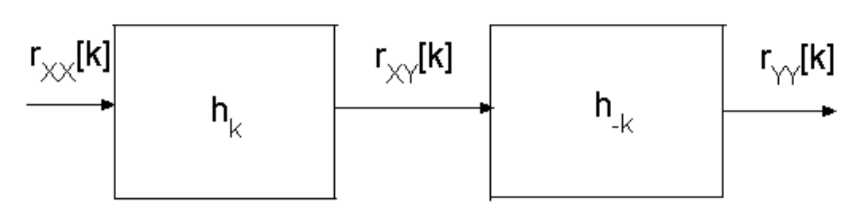
\includegraphics[width = 0.6\textwidth]{lti}
\caption{Correlation functions for a WSS input to a LTI system i.e. $r_{YY}[k] = r_{XX}[k] * h_k * h_{-k}$. Shown easily through the convolution representation.}
\end{centering}
\end{figure}

Converting to the frequency spectrum, 
\begin{align*}
\mathcal{S}_Y(e^{j \omega T}) = |\mathcal{H}(e^{j \omega T})|^2 \mathcal{S}_X(e^{j \omega T})
\end{align*}
Note that $\mathcal{H}(e^{j \omega T}) = \mathcal{Z}[h_k]|_{z=e^{j \omega T}}$; the Z transform and the DTFT are inherently linked.

\item\ix{Ergodicity} Ergodic processes are WSS processes for which statistical characteristics can be obtained through time averages e.g.
\begin{itemize}
\item Mean Ergodic: $\mu = \mathbb{E}[X_n] = \lim_{N\rightarrow\infty} \frac{1}{N} \sum_{n=0}^{N-1}x_n$

\item Correlation Ergodic: $r_{XX}[k] =  \lim_{N\rightarrow\infty} \frac{1}{N} \sum_{n=0}^{N-1}x_nx_{n+k}$
\end{itemize}
and hence the above methods can be used for estimation for sufficiently large $N$. IT is hard to determine whether a process is ergodic; the following rules are used:
\begin{enumerate}
\item Necessary and sufficient condition for mean ergodicity:
\begin{align*}
\lim_{N\rightarrow\infty} \frac{1}{N} \sum_{k=0}^{N-1} c_{XX}[k] = 0
\end{align*}
where $c_{XX}[k]$ is the auto-covariance function. 

\item A sufficient condition for mean ergodicity is that $c_{XX}[0] < \infty $ and $\lim_{N\rightarrow\infty} c_{XX}[n] = 0$.
\end{enumerate}
\textbf{Unless otherwise stated, assume that signals in this course are both wide-sense stationary and ergodic} but this is often not true in practice!!

\item\ix{The Wiener Filter} The Wiener filter is optimally adapted to the statistical characteristics of a random process. A desired signal is hidden is noise:
\begin{align*}
x_n = d_n + v_n
\end{align*}
The Wiener filter is the optimal linear filter for estimation of $d_n$ using $x_n$ with some assumptions regarding the processes. It is assumed that \textbf{$\lbrace x_n \rbrace$ and $\lbrace d_n \rbrace$ are jointly WSS} i.e. all correlation functions are a function of only the time difference. 

Filter derivation:\ix{Derivation}
\begin{enumerate}
\item Depending on the type of filter to be used i.e. order of filter, choose an impulse response for the filter $h_p$.
\item Define $J = \mathbb{E}[\epsilon_n^2]$ where $e_n = d_n - \hat{d_n}$ where $\hat{d_n} = h_p * x_n$.
\item Set $\frac{\partial J}{\partial h_q} = 0$ \textbf{simultaneously for all filter values}. This leads gives the \textbf{orthogonality principle}; 
\begin{align*}
\mathbb{E}[\epsilon_n x_{n-q}] =0\ \forall\ q
\end{align*}
\item Substitute for $\epsilon_n$.

If the filter is finite, this gives an infinite number of equations and is most easily solved in the frequency domain:\ix{Infinite Solution}
\begin{align*}
\mathcal{H}(e^{j \Omega}) \mathcal{S}_X(e^{j \Omega}) = \mathcal{S}_{XD}(e^{j \Omega})
\end{align*}
Where $\mathcal{S}_{XD}(e^{j \Omega})$ is the cross-power spectrum, generally complex valued and measuring the coherence between two processes at a particular frequency. Note that:
\begin{align*}
\mathcal{S}_{XD}(e^{j \Omega}) = \mathcal{S}_{DX}^*(e^{j \Omega})
\end{align*}

\ix{FIR Filter}For an FIR filter, there are a finite number of simultaneous equations which can be solved (e.g. calculating the matrix inverse). 
\begin{align*}
  \vect{R_xh} = \vect{r_{xd}}
\end{align*}
\item Substitute back into $J$, using the orthogonality principle. It is easier to integrate the power spectrum of the error signal over frequencies.  
\end{enumerate}
For an infinite filter with uncorrelated noise, the equations form:
\begin{align*}
\mathcal{H}(e^{j \Omega}) = \frac{\mathcal{S}_{D}(e^{j \Omega})}{\mathcal{S}_{D}(e^{j \Omega})+ \mathcal{S}_{V}(e^{j \Omega})}
\end{align*}

\item\ix{Correlation Matrix}The correlation matrix is often formed when solving the Weiner-Hoff equations.
\begin{align*}
\vect{R}_{X} = \begin{bmatrix}
r_{XX}[0] & r_{XX}[1] & \cdots & r_{XX}[N]\\
r_{XX}[1] & r_{XX}[0] & \cdots & r_{XX}[N-1]\\
\vdots & \vdots & \ddots & \vdots\\
r_{XX}[N] & r_{XX}[N-1] & \cdots & r_{XX}[0]
\end{bmatrix}
\end{align*}
Since $r_{XX}[k]=r_{XX}[-k]$, $\vect{R}_{X}$ is a symmetric matrix and also has constant diagonals. For a generated sequence, $r_{dd}[k]$, the autocorrelation matrix formed must be valid. A necessary condition is that  $\vect{R}_{X}$ is non-negative definite i.e.
\begin{align*}
\vect{a^T R_X a} \geq 0\ \forall \vect{a}
\end{align*}
\textbf{Proof: } Consider $\vect{x_n} = [x_n x_{n-1} ... x_{n-N} ]$ noting that $(\vect{a^T x_n})^2 = \vect{a^T(x_n x_n^T)a} \geq 0$. $\mathbb{E}[x_n x_n^T] = \vect{R_x}$ and take the expectation of the expanded formula where $\vect{a}$ is not random. 

\item\ix{Matched Filters}Whilst the Wiener filter extracts a random filter from noise, \textbf{matched filters are used to detect a known signal buried in noise}.
\begin{align*}
\vect{x = s + v} 
\end{align*}
For a FIR filter with length $N$, the output at $N-1$ can be obtained as a dot product where a tilde represents a time reversed vector. The output has a component due to the deterministic signal as well as the noise. 
\begin{align*}
y_{N-1} = \vect{h^T \tilde{s} + h^T \tilde{v}}
\end{align*}
In order to give the best change of detecting the signal, the SNR is maximised at the output of the filter at this time. 
\begin{align*}
\text{SNR} = \frac{|\vect{h^T \tilde{s}}|^2}{\mathbb{E}[|\vect{h^T \tilde{v}}|^2]} = \frac{\vect{h^T (\tilde{s}\tilde{s}^T) h}}{\mathbb{E}[|\vect{h^T \tilde{v}}|^2]} 
\end{align*}
The matrix $\vect{M = \tilde{s}\tilde{s}^T}$ has eigenvector $\vect{\frac{\tilde{s}}{|\tilde{s}|}}$ with eigenvalue $\vect{\tilde{s}^T\tilde{s}}$. Any other vector orthogonal to this eigenvector i.e. $\vect{\tilde{s}^Tx}=0$ will have eigenvalue zero (by substitution). Hence an orthonormal basis can be formed and using this property simplification made.
\begin{align*}
\vect{h^T (\tilde{s}\tilde{s}^T) h} &= \vect{h^T} \alpha\  (\vect{\tilde{s}^T\tilde{s}}) \frac{\vect{\tilde{s}}}{|\vect{\tilde{s}}|} \\
&= \alpha^2 (\vect{\tilde{s}^T\tilde{s}})
\end{align*}
For a white, zero mean noise process with variance $\sigma_v^2$
\begin{align*}
\mathbb{E}[|\vect{h^T \tilde{v}}|^2] = \sigma_v^2 \vect{h^Th}
\end{align*}
\textbf{Noting that scaling h would not change the SNR, set $|\vect{h}|=1$}. 
\begin{align*}
\text{SNR} = \frac{\alpha^2 (\tilde{s}\tilde{s}^T)}{\sigma_v^2}
\end{align*}
Where $\alpha$ is the the projection of $\vect{h}$ on to $\vect{\tilde{s}}$. The maximum value of $\alpha$ is chosen ($1$). Since the deterministic correlation function is always at a maximum with zero lag, the signal output term for the optimal filter is always less than that computed for $n = N-1$ and hence a maximum is looked for. 

\textbf{Hence the optimal filter is the (normalised), time reversed version of the desired signal.} 

Without using the filter, the maximum achievable SNR is $\frac{\text{max. signal val}}{\sigma_v^2}$ and hence the matched filter gives a significant benefit.

\item\ix{Einstein-Wiener-Khinchin Theorem}For a time windowed signal of length \(2N+1\), \(\vect{x_n^N = w_n^N x_n}\) where 
\begin{align*}
  \vect{w_n^N} = \begin{cases}
    1\ \ \  &-N \leq n \leq N \\
    0 &\text{otherwise}
  \end{cases}
\end{align*}
The DTFT of the windowed signal is effectively the DFT evaluated at continuous frequencies with a origin shift which introduces a linear phase shift. Note that 
\begin{align*}
  \text{DTFT}\mybrace{\vect{x_n^N} * \vect{x_{-n}^N}} &= X^N(e^{j \Omega}) X^N(e^{j \Omega})^* = \magn{X^N(e^{j \Omega})}^2 \\
  \mybrace{\vect{x_n^N} * \vect{x_{-n}^N}}(m) &= \sum_n\vect{x_nw_n^Nx_{n-m}w_{n-m}^N} \\
  \therefore \text{DTFT}\mybrace{\mathbb{E}[\frac{1}{2N+1} \sum_n\vect{x_nw_n^Nx_{n-m}w_{n-m}^N}]} &= \mathbb{E}[\frac{1}{2N+1} \magn{X^N(e^{j \Omega})}^2] \\
  &= r_{XX[m]} \frac{1}{2N+1} \sum_n \vect{w_n^N w_{n-m}^N} \\
  &= r_{XX}[m]t[m]
\end{align*}
noting the linearity of the DTFT and expectation. \(t[m]\) is the deterministic autocorrelation function of the window function, $w_n$. As $n$ increases, $t[m]$ gives wider and flatter and hence $T(e^{j\Omega})$ tends towards a delta function. 

\begin{align*}
  \text{DTFT}\mybrace{r_{XX}[m]t[m]} = \mathcal{S}_X(e^{j\Omega}) * T(e^{j\Omega}) &= \mathbb{E}[\frac{1}{2N+1} \magn{X^N(e^{j \Omega})}^2] \\
  \lim_{N\rightarrow\infty} \mathbb{E}[\frac{1}{2N+1} \magn{X^N(e^{j \Omega})}^2] &= \mathcal{S}_X(e^{j\Omega})
\end{align*}
Hence the power spectrum\ix{Interpretation} can be understood as the expected value of (time-normalised) DTFT squared of the signal values. Hence, the a random DFT/DTFT should look similar to the underlying power spectrum of the process.

\item\ix{Estimation Setup}In general, a set of unknown parameters are inferred from a a number of measurements i.e. where $P<<N$
\begin{align*}
  \vect{x} = \begin{bmatrix}
    x_0 \\ x_1 \\ \vdots \\ x_{N-1}
  \end{bmatrix}
  \hspace{1cm}
  \vect{\theta} = \begin{bmatrix}
    \theta_0 \\ \theta_1 \\ \vdots \\ \theta_{P-1}
  \end{bmatrix}
\end{align*}
We will assume that we are able to model the probability of receiving the given data, $\vect{x}$, given the parameters i.e. $p(\vect{x}|\vect{\theta})$ is known. Note that \textbf{estimation seeks to estimate a single value whilst the task of inference is to infer the entire probability distribution}.

\item\ix{Assessing Estimator}There are multiple methods to estimating a parameter such as the mean of a population. In order to assess estimators, we must consider:
\begin{enumerate}
  \item Estimator \textbf{bias}. If \(\hat{\mu}\) is an estimator, consider whether
  \begin{align*}
    \mathbb{E}[\hat{\mu}] = \mu = \mathbb{E}[X]
  \end{align*}
  If true, the estimator is said to be unbiased. 
  \item Estimator \textbf{variance}
  \begin{align*}
    \text{Var}[\hat{\mu}] = \mathbb{E}[\hat{\mu}^2] - \mathbb{E}[\hat{\mu}]^2
  \end{align*}
  The variance measures how the likely spread of the estimator; if the variance is large, even if unbiased, a typical estimate may be far from the true value.
\end{enumerate}

An unbiased estimator whose variance tends to \(0\) as \(N \rightarrow \infty \) is said to be \textbf{consistent} and given enough data will get the `correct' estimate. The best estimator for a specific problem has no bias and the minimum variance is the \emph{MVU (minimum variance ubiased) estimator}.


\item\ix{The Geneal Linear Model}In the linear model, it is assumed that the data is generated as some linear function of the parameters with an added noise term i.e.
\begin{align*}
  x_n = \vect{g_n^T}\vect{\theta} + e_n &\hspace{1cm}\text{or } \vect{x = G}\vect{\theta} + \vect{e} \text{ where}\\
  \vect{G} = &\begin{bmatrix}
    \vect{g_0^T} \\
    \vect{g_1^T} \\
    \vdots\\
    \vect{g_{N-1}^T}
  \end{bmatrix}
\end{align*}
$\vect{G}$ can be chosen to give a wide of possible models and may be fixed after the data has been observed (but in this case, the data cannot be generated from the model). The order of the model is the number of parameters in the model.

\item\ix{Ordinary Least Squares Estimation}The OLS estimator finds a `best fit' model which matches the data by minimising
\begin{align*}
  J = \vect{e}^T\vect{e}
\end{align*}
i.e. the least squared error. For the general linear model, a pseudo-inverse solution is reached
\begin{align*}
  \vect{\theta}^{OLS} = (\vect{G}^T\vect{G})^{-1}\vect{G}^T\vect{x}
\end{align*}
which can be obtained by setting \(\frac{\partial J}{\partial \vect{\theta}} = \vect{0}\) (note the vector \(\vect{0}\)) or by completing the square which shows that the OLS estimator is \textbf{globally} optimal. 

It can be shown that the OLS estimator is unbiased easily through substitution into the relevant equations.\ix{Covariance of OLS} The variance is more difficult to consider. Define the OLS matrix term as \(\vect{C}=(\vect{G}^T\vect{G})^{-1}\vect{G}^T\) and examine the variance of \textbf{any other unbiased estimator}, \(\vect{\hat{\theta}}\). 
\begin{align*}
  \vect{\hat{\theta}} = \vect{Dx} \hspace{1cm} \vect{D} = \vect{C} +  \vect{\Delta}
\end{align*}
\(\vect{\Delta}\) is some matrix perturbation away from the OLS solution. 
\begin{align*}
  \expt{\vect{Dx}} &= \expt{\vect{(C + \Delta)x}} = 
  \vect{\theta + \Delta G \theta} = \vect{\theta} \\
  \therefore\ &\vect{\Delta G=0} \text{ since true for all } \vect{\theta}
\end{align*}
Define the covariance matrix for the estimator
\begin{align*}
  \text{cov}(\vect{\hat{\theta}}) = \expt{(\vect{\hat{\theta}} - \expt{\vect{\hat{\theta}}}) (\vect{\hat{\theta}} - \expt{\vect{\hat{\theta}}})^T} = \expt{ \vect{\hat{\theta}} \vect{\hat{\theta}}^T} - \vect{\theta}\vect{\theta}^T
\end{align*}

note that the \((i, i)\)th element is the variance of \(\hat{\theta_i}\) and the simplification is due to the estimators being unbiased. Assume that the error is \textbf{zero mean white noise with variance} \(\sigma_e^2\). Using this, substituting in \(\vect{\hat{\theta}}, \vect{D}\) and using \(\vect{\Delta G=0}\)
\begin{align*}
  \text{cov}(\vect{\hat{\theta}}) = \expt{\vect{\hat{\theta}}\vect{\hat{\theta}}^T} - \vect{\theta}\vect{\theta}^T = \sigma_e^2\vect{DD}^T
\end{align*}
Expanding \(\vect{D}\) out and noting that \(\vect{\Delta C}^T=\vect{C\Delta}^T=\vect{0}\) we  form
\begin{align*}
  \text{cov}(\vect{\hat{\theta}}) &= \sigma_e^2 ((\vect{G}^T\vect{G})^{-1} + \vect{\Delta \Delta}^T) \\
  &= \text{cov}(\vect{\theta}^{OLS}) + \sigma_e^2 \vect{\Delta \Delta}^T
\end{align*}
The diagonal elements of \(\vect{\Delta \Delta}\) are \(\geq 0\) with equality corresponding to the OLS solution. Therefore \(\text{var}(\hat{\theta_i})\geq \text{var}(\theta_i^{OLS})\) and hence the OLS estimator is the minimum variance unbiased estimator of \(\vect{\theta}\) and is termed a \textbf{best linear unbiased estimator (BLUE)}.\ix{Blue}

\item\ix{Likelihood Estimation}If he error sequence is assumed drawn from an iid source whose probability distribution is known, likelihood estimation may be used. 
\begin{align*}
  p(\vect{e}) = p_e(e_0)p_1(e_1)\ldots p_e(e_{N-1})
\end{align*}
If \(p_e\) is the zero-mean normal distribution, the model is equivalent to the Linear Gaussian model. \textbf{Choose the value of} \(\vect{\theta}\) \textbf{which maximises the likelihood of the observed data,} \vect{x} i.e.
\begin{align*}
  \vect{\theta}^{ML} = \arg\max_{\vect{\theta}}\mybrace{p(\vect{x}|\vect{\theta})} 
\end{align*}
This can be achieved using standard differential calculus. It is often convenient to maximise the log-likelihood function since it is a monotonically increasing function. In the case of the Linear Gaussian model, the \textbf{the least squares solution is equivalent to the maximum likelihood solution}.

The noise variance can also be estimated by considering the log-likelihood function at the optimal parameter estimate. The noise level is the mean-squared error at the ML parameter solution.


\item\ix{Bayesian Method}If the parameters are treated as random vectors with pdfs assigned to the parameters which \textbf{represent some prior knowledge about the relative probability of different parameters before the data is observed}. If nothing is known \emph{a priori} then the prior distributions should express no intial preferences. 

\begin{align*}
  p(\vect{\theta}|\vect{x}) = \frac{p(\vect{x}|\vect{\theta})p(\vect{\theta})}{p(\vect{x})} \propto p(\vect{x}|\vect{\theta})p(\vect{\theta})
\end{align*}
\(p(\vect{\theta}|\vect{x})\) is termed the posterior probability whilst \(p(\vect{\theta})\) is termed the prior. The posterior probability is made up of the `new information' from the data and the prior belief of the data which may even be highly subjective. The \textbf{prior should be chosen carefully}. Note that the marginal likelihood, \(p(\vect{x})\) can be obtained through marginalisation. 

Note that we are also implicitly conditioning on many pieces of additional prior information e.g.\ the form of the data generation process. To reflect this, the prior is occasionally written as \(p(\vect{\theta}|\vect{x}, \mathcal{M})\) where \(\mathcal{M}\) denotes all of the additional modelling and distribution assumptions made. 

\begin{align*}
  \vect{\theta}^{\text{MAP}} = \arg \max_{\vect{\theta}} \mybrace{ p(\vect{\theta}|\vect{x})}
\end{align*}

The ML estimate can be interpreted as the MAP estimate with a uniform prior. As the sample size tends towards infinity, the Bayesian solution tends towards the maximum likelihood solution.

Note that the Gaussian is said to be a `conjugate' prior since it's form makes Bayesian calculations straightforward and available in closed form. 


\item\ix{MMSE}Extending the Bayesian approach, alternatively, a cost function could be minimised, \(C(\vect{\hat{\theta}}, \vect{\theta})\) which expresses the cost of an incorrect estimation. This is usually a non-negative function with \(C(\vect{\theta}, \vect{\theta})=0\). Then solve
\begin{align*}
  \min_{\vect{\hat{\theta}}} \expt{C(\vect{\hat{\theta}}, \vect{\theta})} \hspace{1cm} \hat{\vect{\theta}}\vect{(x)}
\end{align*}
If only one parameter is being estimated and \(C(\hat{\theta}, \theta)=(\hat{\theta}-\theta)^2\), differentiation leads to the following result:
\begin{align*}
  \hat{\theta}^{\text{MMSE}} = \expt{\theta|\vect{x}}
\end{align*}
For the linear gaussian model, the estimator coincides with the \emph{maximum a posteriori} estimator but this is not always the case. 

\end{enumerate}
\end{document}